\chapter{Introduction}

\begin{figure*}
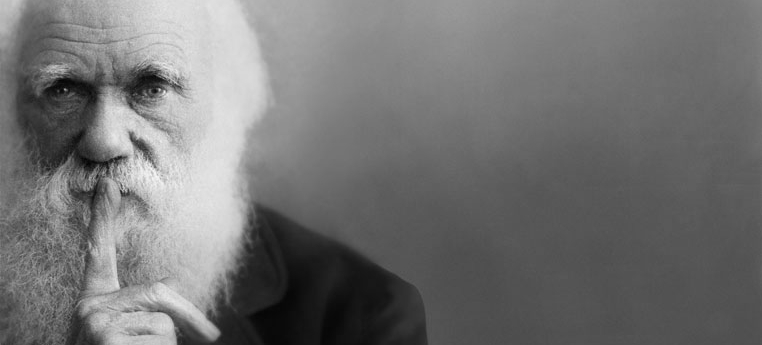
\includegraphics[width=\textwidth]{Images/DarwinWide.jpg}
\caption{Charles Darwin}
\end{figure*}

\lettrine[lines=3,slope=0pt,findent=0pt]{W}{hen} on board H.M.S. 'Beagle,' as naturalist, I was much struck with certain facts in the distribution of the inhabitants of South America, and in the geological relations of the present to the past inhabitants of that continent. These facts seemed to me to throw some light on the origin of species--that mystery of mysteries, as it has been called by one of our greatest philosophers. On my return home, it occurred to me, in 1837, that something might perhaps be made out on this question by patiently accumulating and reflecting on all sorts of facts which could possibly have any bearing on it. After five years' work I allowed myself to speculate on the subject, and drew up some short notes; these I enlarged in 1844 into a sketch of the conclusions, which then seemed to me probable: from that period to the present day I have steadily pursued the same object. I hope that I may be excused for entering on these personal details, as I give them to show that I have not been hasty in coming to a decision.
My work is now nearly finished; but as it will take me two or three more years to complete it, and as my health is far from strong, I have been urged to publish this Abstract. I have more especially been induced to do this, as Mr. Wallace\footnote{Alfred Russel Wallace was a British naturalist, explorer, geographer, anthropologist, and biologist. He is best known for independently conceiving the theory of evolution through natural selection.}, who is now studying the natural history of the Malay archipelago, has arrived at almost exactly the same general conclusions that I have on the origin of species. Last year he sent to me a memoir on this subject, with a request that I would forward it to Sir Charles Lyell, who sent it to the Linnean Society, and it is published in the third volume of the Journal of that Society. Sir C. Lyell and Dr. Hooker, who both knew of my work--the latter having read my sketch of 1844--honoured me by thinking it advisable to publish, with Mr. Wallace's excellent memoir, some brief extracts from my manuscripts.
This Abstract, which I now publish, must necessarily be imperfect. I cannot here give references and authorities for my several statements; and I must trust to the reader reposing some confidence in my accuracy. No doubt errors will have crept in, though I hope I have always been cautious in trusting to good authorities alone. I can here give only the general conclusions at which I have arrived, with a few facts in illustration, but which, I hope, in most cases will suffice. No one can feel more sensible than I do of the necessity of hereafter publishing in detail all the facts, with references, on which my conclusions have been grounded; and I hope in a future work to do this. For I am well aware that scarcely a single point is discussed in this volume on which facts cannot be adduced, often apparently leading to conclusions directly opposite to those at which I have arrived. A fair result can be obtained only by fully stating and balancing the facts and arguments on both sides of each question; and this cannot possibly be here done.
I much regret that want of space prevents my having the satisfaction of acknowledging the generous assistance which I have received from very many naturalists, some of them personally unknown to me. I cannot, however, let this opportunity pass without expressing my deep obligations to Dr. Hooker, who for the last fifteen years has aided me in every possible way by his large stores of knowledge and his excellent judgment.
In considering the Origin of Species, it is quite conceivable that a naturalist, reflecting on the mutual affinities of organic beings, on their embryological relations, their geographical distribution, geological succession, and other such facts, might come to the conclusion that each species had not been independently created, but had descended, like varieties, from other species. Nevertheless, such a conclusion, even if well founded, would be unsatisfactory, until it could be shown how the innumerable species inhabiting this world have been modified, so as to acquire that perfection of structure and coadaptation which most justly excites our admiration. Naturalists continually refer to external conditions, such as climate, food, etc., as the only possible cause of variation. In one very limited sense, as we shall hereafter see, this may be true; but it is preposterous to attribute to mere external conditions, the structure, for instance, of the woodpecker, with its feet, tail, beak, and tongue, so admirably adapted to catch insects under the bark of trees. In the case of the misseltoe, which draws its nourishment from certain trees, which has seeds that must be transported by certain birds, and which has flowers with separate sexes absolutely requiring the agency of certain insects to bring pollen from one flower to the other, it is equally preposterous to account for the structure of this parasite, with its relations to several distinct organic beings, by the effects of external conditions, or of habit, or of the volition of the plant itself.
The author of the 'Vestiges of Creation' would, I presume, say that, after a certain unknown number of generations, some bird had given birth to a woodpecker, and some plant to the misseltoe, and that these had been produced perfect as we now see them; but this assumption seems to me to be no explanation, for it leaves the case of the coadaptations of organic beings to each other and to their physical conditions of life, untouched and unexplained.
It is, therefore, of the highest importance to gain a clear insight into the means of modification and coadaptation. At the commencement of my observations it seemed to me probable that a careful study of domesticated animals and of cultivated plants would offer the best chance of making out this obscure problem. Nor have I been disappointed; in this and in all other perplexing cases I have invariably found that our knowledge, imperfect though it be, of variation under domestication, afforded the best and safest clue. I may venture to express my conviction of the high value of such studies, although they have been very commonly neglected by naturalists.
From these considerations, I shall devote the first chapter of this Abstract to Variation under Domestication. We shall thus see that a large amount of hereditary modification is at least possible, and, what is equally or more important, we shall see how great is the power of man in accumulating by his Selection successive slight variations. I will then pass on to the variability of species in a state of nature; but I shall, unfortunately, be compelled to treat this subject far too briefly, as it can be treated properly only by giving long catalogues of facts. We shall, however, be enabled to discuss what circumstances are most favourable to variation. In the next chapter the Struggle for Existence amongst all organic beings throughout the world, which inevitably follows from their high geometrical powers of increase, will be treated of. This is the doctrine of Malthus, applied to the whole animal and vegetable kingdoms. As many more individuals of each species are born than can possibly survive; and as, consequently, there is a frequently recurring struggle for existence, it follows that any being, if it vary however slightly in any manner profitable to itself, under the complex and sometimes varying conditions of life, will have a better chance of surviving, and thus be NATURALLY SELECTED. From the strong principle of inheritance, any selected variety will tend to propagate its new and modified form.
This fundamental subject of Natural Selection will be treated at some length in the fourth chapter; and we shall then see how Natural Selection almost inevitably causes much Extinction of the less improved forms of life and induces what I have called Divergence of Character. In the next chapter I shall discuss the complex and little known laws of variation and of correlation of growth. In the four succeeding chapters, the most apparent and gravest difficulties on the theory will be given: namely, first, the difficulties of transitions, or in understanding how a simple being or a simple organ can be changed and perfected into a highly developed being or elaborately constructed organ; secondly the subject of Instinct, or the mental powers of animals, thirdly, Hybridism, or the infertility of species and the fertility of varieties when intercrossed; and fourthly, the imperfection of the Geological Record. In the next chapter I shall consider the geological succession of organic beings throughout time; in the eleventh and twelfth, their geographical distribution throughout space; in the thirteenth, their classification or mutual affinities, both when mature and in an embryonic condition. In the last chapter I shall give a brief recapitulation of the whole work, and a few concluding remarks.

\begin{figure}
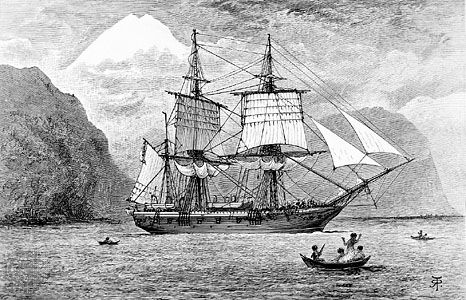
\includegraphics[width=\linewidth]{Images/HMSBeagle.jpg}
\caption{H.M.S. Beagle}
\end{figure}

No one ought to feel surprise at much remaining as yet unexplained in regard to the origin of species and varieties, if he makes due allowance for our profound ignorance in regard to the mutual relations of all the beings which live around us. Who can explain why one species ranges widely and is very numerous, and why another allied species has a narrow range and is rare? Yet these relations are of the highest importance, for they determine the present welfare, and, as I believe, the future success and modification of every inhabitant of this world. Still less do we know of the mutual relations of the innumerable inhabitants of the world during the many past geological epochs in its history. Although much remains obscure, and will long remain obscure, I can entertain no doubt, after the most deliberate study and dispassionate judgment of which I am capable, that the view which most naturalists entertain, and which I formerly entertained--namely, that each species has been independently created--is erroneous. I am fully convinced that species are not immutable; but that those belonging to what are called the same genera are lineal descendants of some other and generally extinct species, in the same manner as the acknowledged varieties of any one species are the descendants of that species. Furthermore, I am convinced that Natural Selection has been the main but not exclusive means of modification.~\\ \\ \hspace*{0pt} ~\hfill  -- Charles Darwin